\documentclass{exam}
\usepackage{main}
\usepackage{graphicx}

\qformat{\textbf{Exercice \thequestion :}\hfill}

\begin{document}
\begin{questions}
\question On considère un champ $ABCD$ de longueur $AB = 100$ mètres et de largeur $BC = 80$. On réduit sa longueur de $x$ mètres et on augmente sa largueur de $x$ mètres aussi. On cherche pour quelle valeurs de $x$ la surface du champ augmente.
\begin{center}
\begin{tikzpicture}
\coordinate (A) at (0,0);
\coordinate (B) at (0,5);
\coordinate (C) at (4,5);
\coordinate (D) at (4,0);
\coordinate (A') at (0,1);
\coordinate (C') at (5,5);
\coordinate (E) at (5,1);
\draw (A) node[left] {$A$};
\draw (B) node[above] {$B$};
\draw (C) node[above] {$C$};
\draw (D) node[right] {$D$};
\draw (A') node[left] {$A'$};
\draw (C') node[above] {$C'$};
\draw (E) node[right] {$E$};
\draw (A) -- (B) -- (C) -- (D) -- cycle;
\draw (A') -- (B) -- (C') -- (E) -- cycle;
\end{tikzpicture}
\end{center}
\begin{parts}
\part Ajouter sur la figure les longueurs données par le problème.
\part Ecrire l'expression de l'aire de la surface $A'BC'E$. Montrer que cette expression est égale à
\begin{equation*}
-x^2 + 20x + 8000
\end{equation*}
\part Donner l'aire de cette surface pour $x = 1$, et pour $x = 5$. Ces valeurs résolvent-elles le problème.
\part Montrer que le problème revient à résoudre l'inéquation
\begin{equation*}
20x - x^2 > 0 
\end{equation*}
\part La courbe représentative de la fonction $f : x \mapsto 20x - x^2$ est donnée ci-après :
\begin{center}
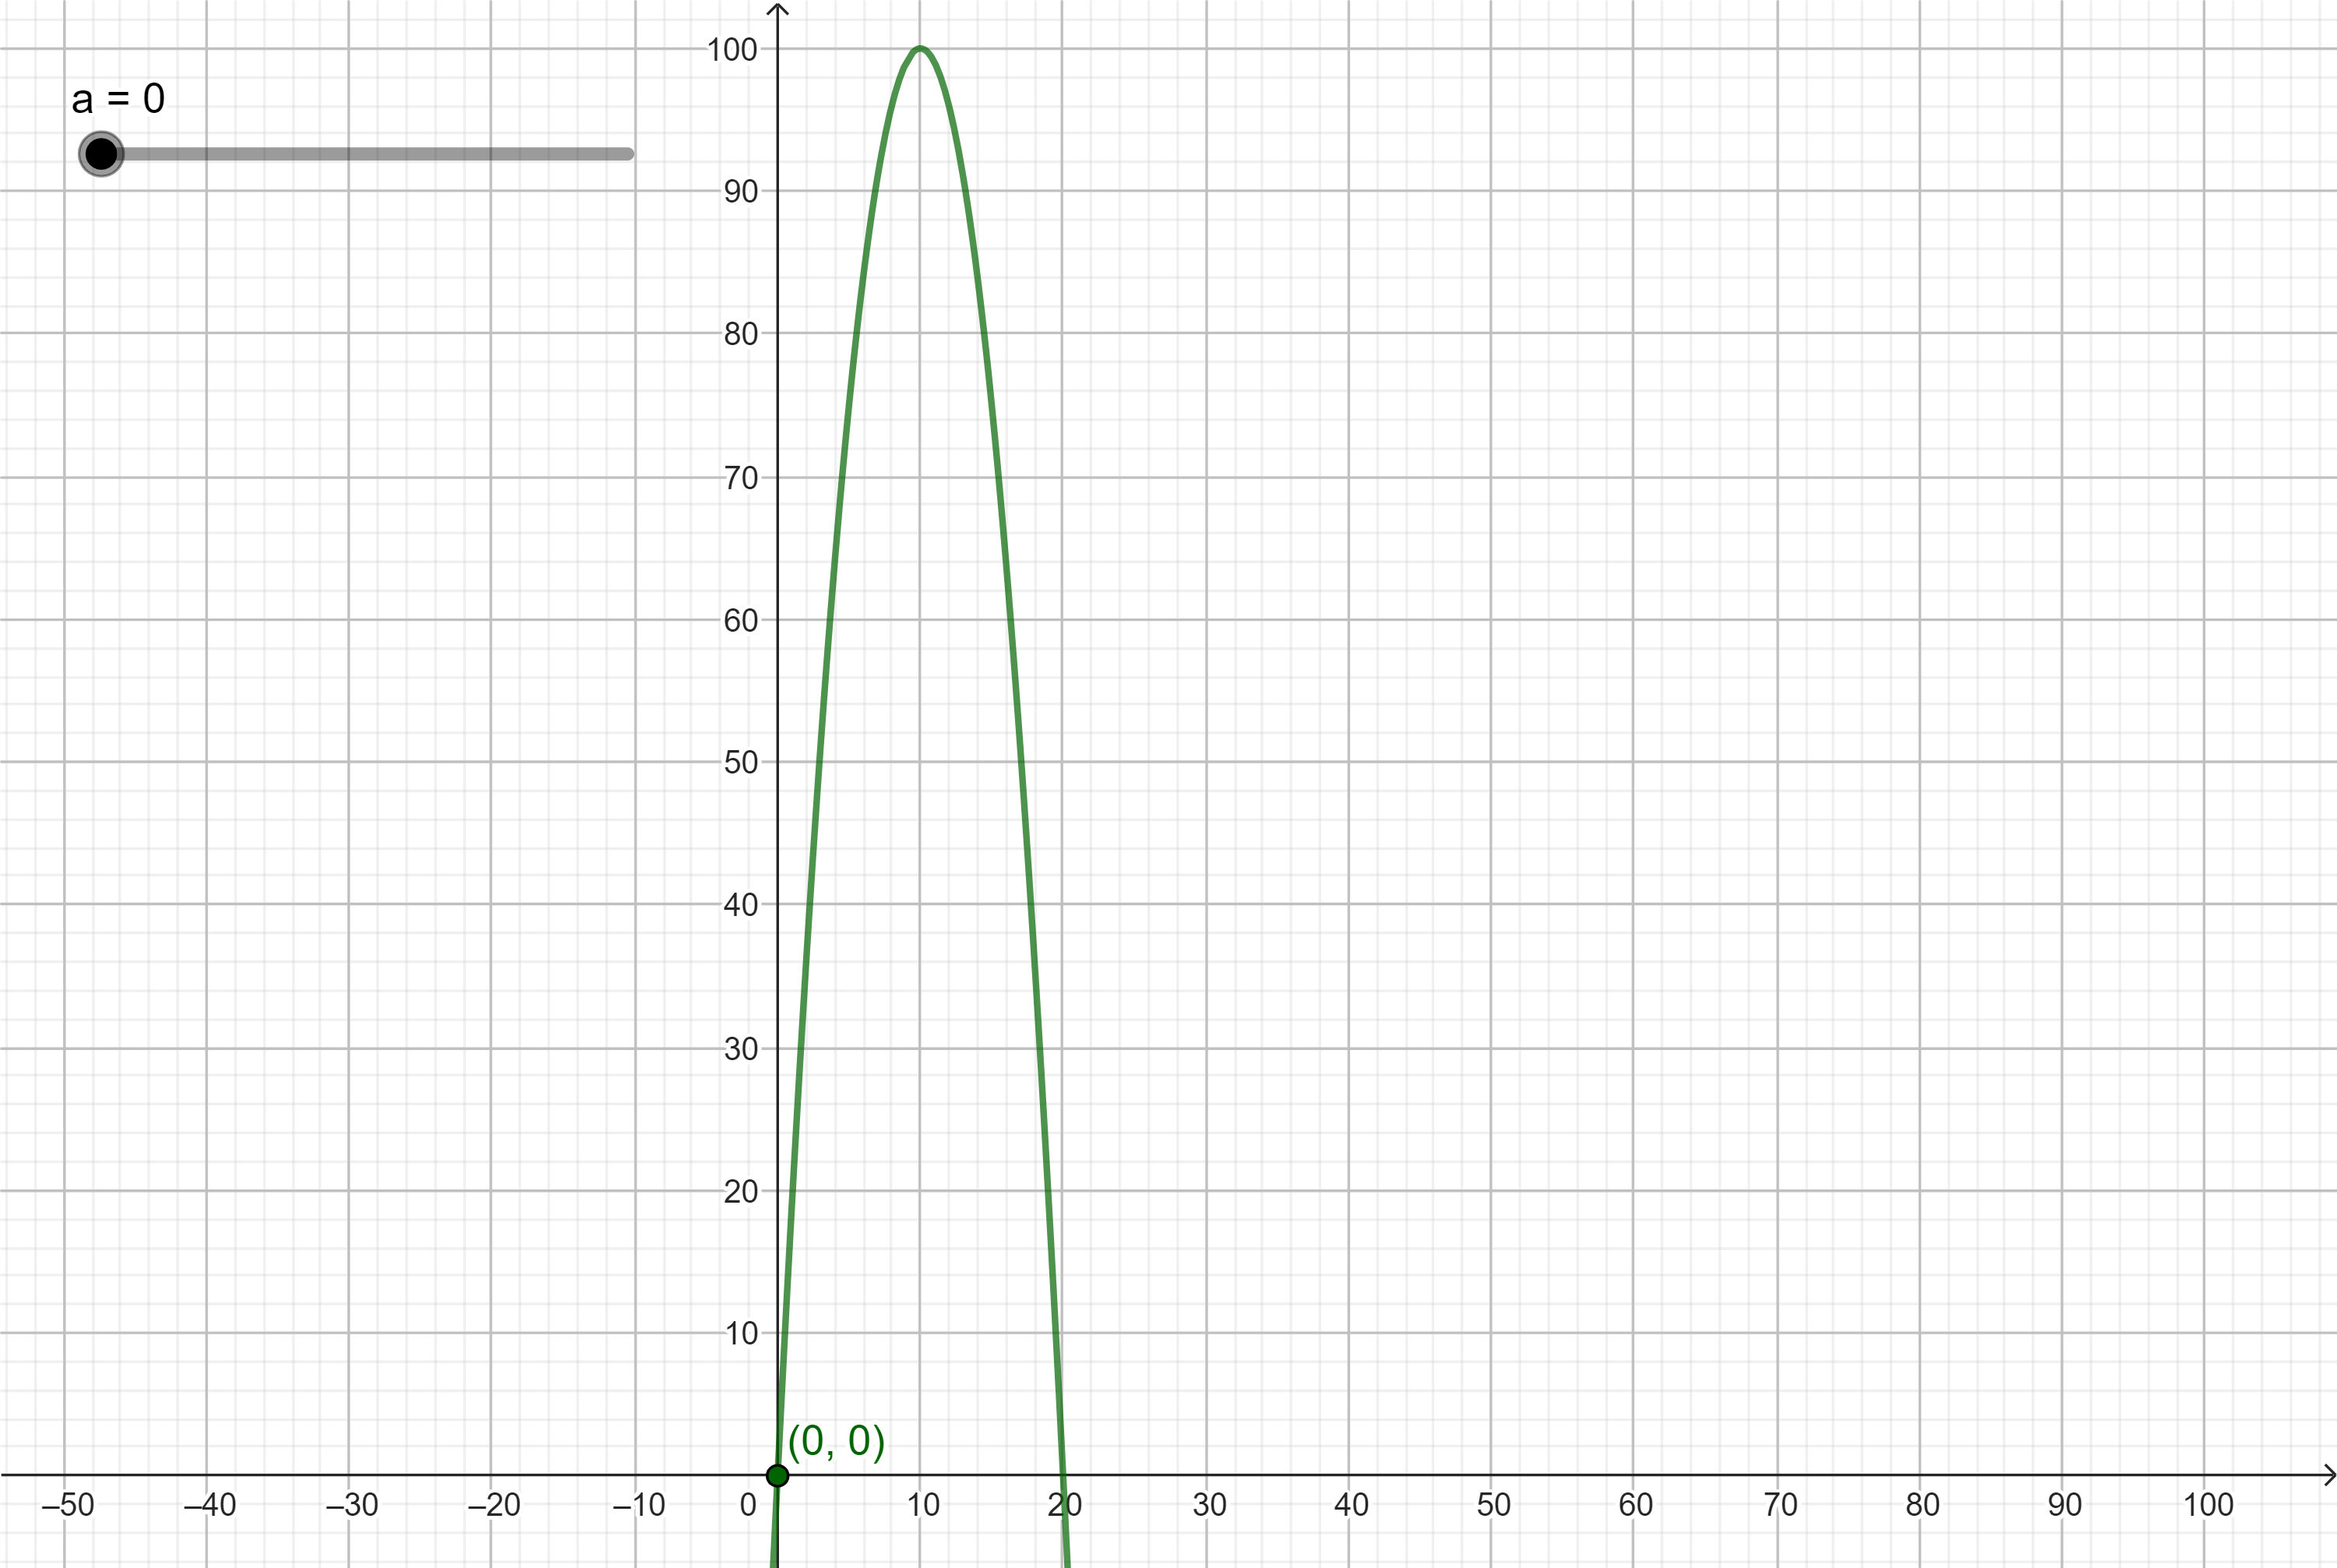
\includegraphics[scale=0.07]{courbe.png}
\end{center}
En déduire l'ensemble des solutions de l'inéquation.
\end{parts}
\end{questions}
\end{document}